\documentclass[fleqn]{beamer}

\usepackage{amsmath,amssymb}
\usepackage{graphicx}
\usepackage{fontspec}
\usepackage{comment}
\usepackage{amsmath, mathtools}
\usepackage{fontspec,xgreek,polyglossia}

\usepackage{graphicx}
\usepackage{float}
\usepackage{hyperref}
\usepackage{url}
\usepackage{siunitx}
\usepackage{caption}
\usepackage{subfigure}
\usepackage{listings}

\renewcommand{\lstlistingname}{Έξοδος προγράμματος}

\hypersetup{
    colorlinks,
    citecolor=black,
    filecolor=black,
    linkcolor=black,
    urlcolor=black
}

\hypersetup{
    colorlinks=true,
    linkcolor=blue,
    filecolor=magenta,      
    urlcolor=cyan,
    bookmarks=true,
    pdfpagemode=FullScreen,
}

\graphicspath{ {./images/} }
\defaultfontfeatures{Mapping=tex-text}

%\setmainfont{Times New Roman}
\setmainfont{CMU Serif}
\setsansfont{CMU Sans Serif}
\setdefaultlanguage[variant=modern]{greek}
\setotherlanguage{english}

% vertical separator macro
\newcommand{\vsep}{
  \column{0.0\textwidth}
    \begin{tikzpicture}
      \draw[very thick,black!10] (0,0) -- (0,7.3);
    \end{tikzpicture}
}

% More space between lines in align
\setlength{\mathindent}{0pt}

% Beamer theme
\usetheme{ZMBZFMK}
% \usefonttheme[onlysmall]{structurebold}
\mode<presentation>
\setbeamercovered{transparent=10}

% align spacing
\setlength{\jot}{0pt}

%\setbeamertemplate{navigation symbols}{}%remove navigation symbols

\title{Ενσωματωμένο Σύστημα Αντί-Mπλοκαρίσματος Τροχών (ABS)}
\author{Σταυρόπουλος Σπύρος, Συμεωνίδης Θεόδωρος}
\institute{Τμήμα Μηχανικών Η/Υ & Πληροφορικής, Πανεπιστήμιο Πατρών}
\date{\today}

\begin{document}

\begin{frame}
  \titlepage
\end{frame}

\begin{frame}
  \frametitle{ABS}
  \begin{columns}[T]
  
    \column{0.5\textwidth}
    
   \begin{itemize}
    \item Σύνθετο σύστημα
    \item Αποτελείται από υδραυλικά, μηχανικά και ηλεκτρικά μέρη.
    \item  Προσφέρει:
        \begin{itemize}
            \item Περισσότερο έλεγχο του τιμονιού στη πέδηση
            \item Συνήθως μειώνει το χρόνο πέδησης
        \end{itemize}
    \end{itemize}

    \column{0.5\textwidth}
    
    \begin{figure}[H]
    \begin{center}
    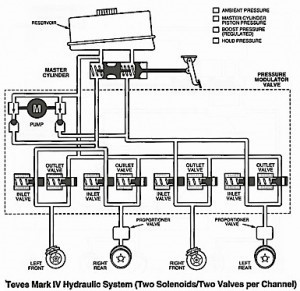
\includegraphics[scale=0.60]{images/hydraulic-mechanical-system-overview.jpg}
    \end{center}
    \end{figure}
    
  \end{columns}
\end{frame}

\begin{frame}
  \frametitle{Περιγραφή προβλήματος}
  \begin{itemize}
      \item Κίνηση χωρίς ολίσθηση $V = \omega \times R$
      \item Σε συνθήκες απότομης πέδησης έχω ολίσθηση δηλ. $V > \omega \times R$
      \item Τότε εμφανίζεται τριβή ολίσθησης αντίρροπη του $V$ που τείνει να εξαλείψει την ανισορροπία, δηλ. να μειώσει το $V$ και να αυξήσει το $\omega$
      \item Κατά τη διαδικασία αυτή χάνει ενέργεια το σύστημα
      \item Θέλουμε τη μέγιστη απώλεια ενέργειας που επιτυγχάνεται για διαφορετικό συντελεστή ολίσθησης $S$ σε κάθε επιφάνεια.
  \end{itemize}
      \begin{figure}[H]
        \begin{center}
        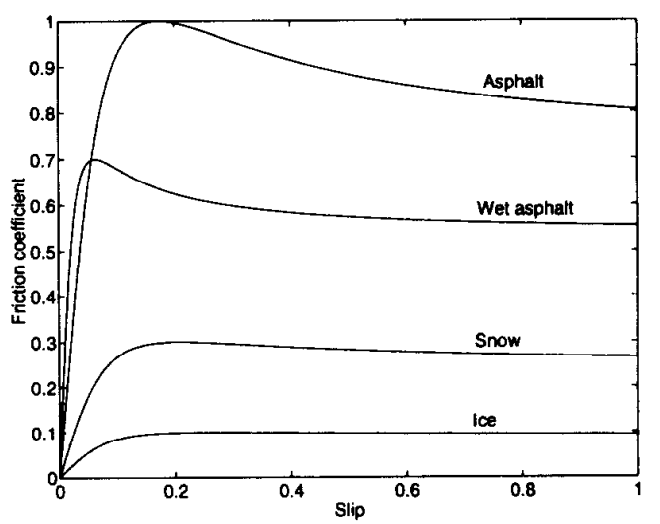
\includegraphics[scale=0.2]{images/slip-friction-diagram.png}
        \end{center}
    \end{figure}
\end{frame}

\begin{frame}
  \frametitle{Λειτουργικές απαιτήσεις χρήστη}
  \begin{itemize}
      \item Nα ενεργοποιείται μόνο σε καταστάσεις πολύ απότομης πέδηση καθώς προκαλεί ολίσθηση που φθείρει τα ελαστικά
      \item Να αποκρίνεται στον ελάχιστο δυνατό χρόνο
      \item Aξιόπιστο, προβλέψιμο, να μπορεί να λειτουργείσε εύρος συνθηκών
      \item Nα προσφέρει κατά τοδυνατό περισσότερο έλεγχο του τιμονιού
  \end{itemize}
\end{frame}

\begin{frame}
  \frametitle{Προδιαγραφές συστήματος}
  \begin{itemize}
      \item Μεγάλη αξιοπιστία σε μεγάλο εύρος συνθηκών οδοστρώματος
      \item Επεξεργαστές υψηλής συχνότητας λειτουργίας και δειγματοληψίας
      \item Δυνατότητα λήψης αποφάσεων τουλάχιστον 10 φορές το δευτερόλεπτο
      \item Δυνατότητα για κάθε τροχό να μπορούμε ξεχωριστά1να αποκόπτουμε/ελευθερώνουμε την πίεση των υδραυλικών
      \item Εύκολη τοποθέτηση και συντήρηση
  \end{itemize}
\end{frame}

\begin{frame}
\frametitle{Προσέγγιση λογισμικού}
\begin{figure}[H]
    \begin{center}
    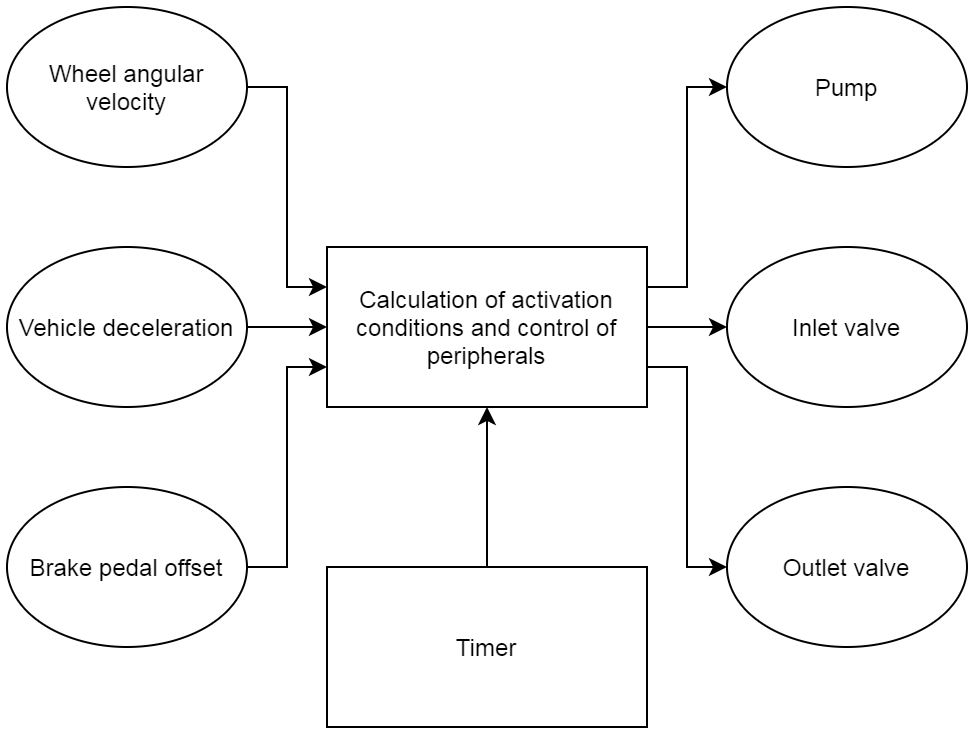
\includegraphics[scale=0.20]{images/software-architecture-preview.png}
    \end{center}
\end{figure}
\end{frame}

\begin{frame}
  \frametitle{Προσέγγιση υλικού}
  \begin{figure}[H]
    \begin{center}
    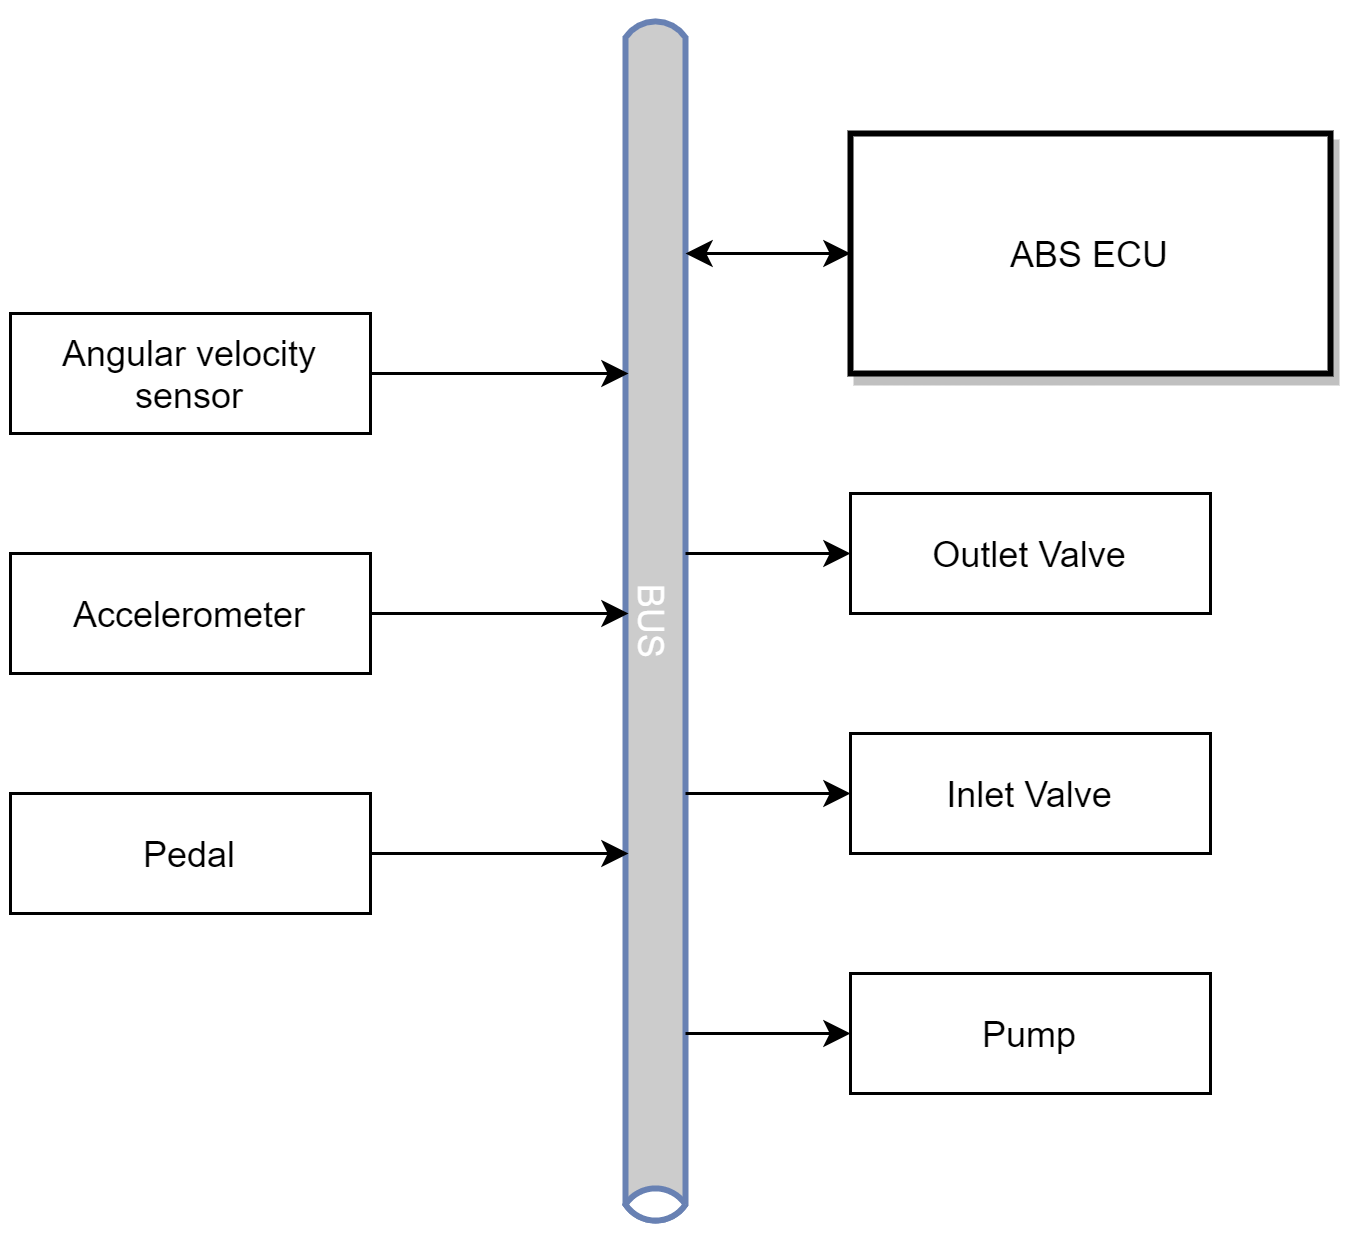
\includegraphics[scale=0.15]{images/hardware-architecture-preview.png}
    \end{center}
\end{figure}
\end{frame}

\begin{frame}
  \frametitle{Αλγόριθμος}
  \begin{itemize}
  \item Βαθιά μελετημένο πρόβλημα τις θεωρίας ελέγχου
  \item Καθορίζει :
  \begin{itemize}
      \item Πότε και κατά πόσο θα πρέπει να αυξάνεται/μειώνεται η πέδηση των τροχών και κατά συνέπεια 
      \item Πότε θα ενεργοποιούνται/απενεργοποιούνται τα επιμέρους υποσυστήματα που το κάνουν πράξη
  \end{itemize}
  \item Επιλέχθηκε ένας αλγόριθμος ασαφούς ελέγχου που προτάθηκε από τον G. F. Mauer και απαιτεί :
  \begin{itemize}
    \item Γωνιακή ταχύτητα (δηλ. αισθητήρες γωνιακής ταχύτητας στους τροχούς)
    \item Επιτάχυνση οχήματος (δηλ. επιταχυνσιόμετρο στο όχημα)
    \item Μνήμη (δηλ. χρονικά μεταβαλλόμενο σύστημα)
  \end{itemize}
  
  \end{itemize}
\end{frame}

\begin{frame}
  \frametitle{Αρχιτεκτονική συστήματος}
  \begin{itemize}
   \item Η αναλυτική αρχιτεκτονική του συστήματος βρίσκεται   \href{https://drive.google.com/file/d/1vFFA7gmCW2vK_F3lPBO-nykZZAyVAGi6/view?usp=sharing}{εδώ} 
  \end{itemize}
  \begin{figure}[h]
    \begin{center}
    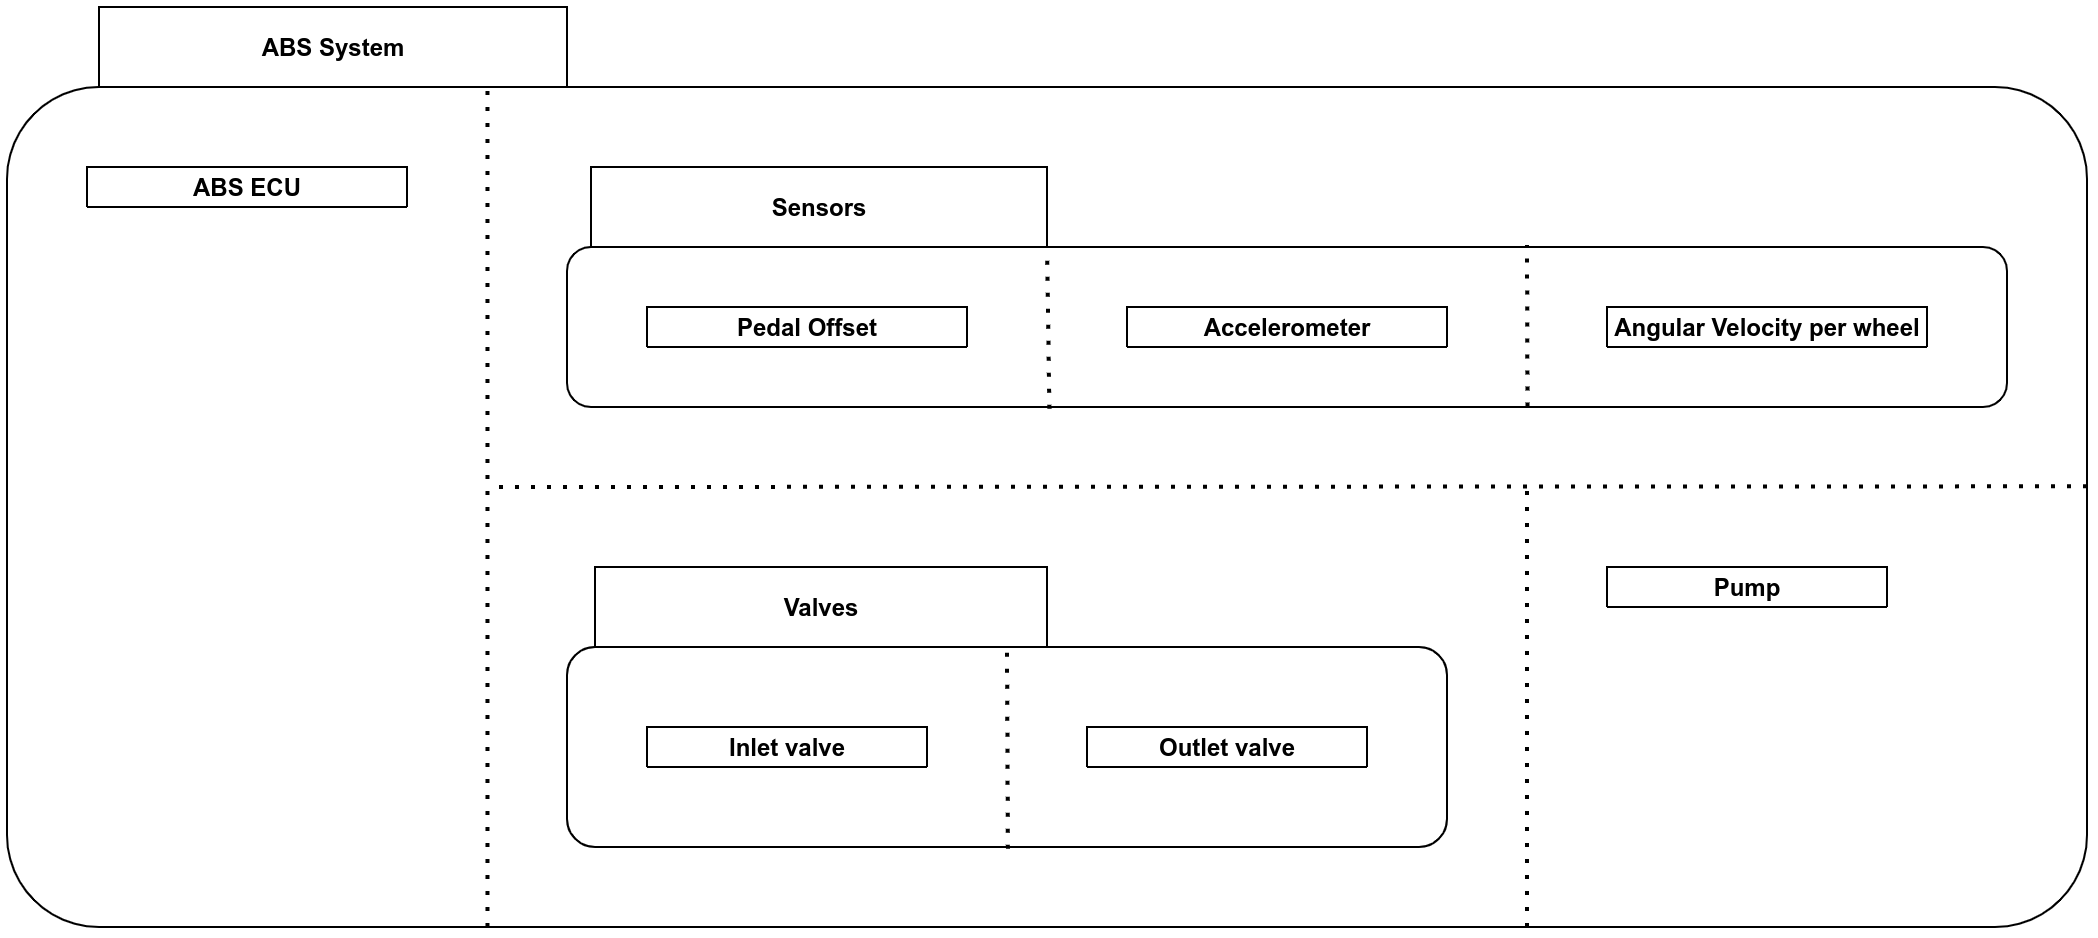
\includegraphics[scale=0.15]{images/system-architecture-overview.png}
    \end{center}
  \end{figure}
\end{frame}

\begin{frame}
  \frametitle{Αρχιτεκτονική λογισμικού}
  \begin{figure}[H]
    \makebox[\textwidth][c]{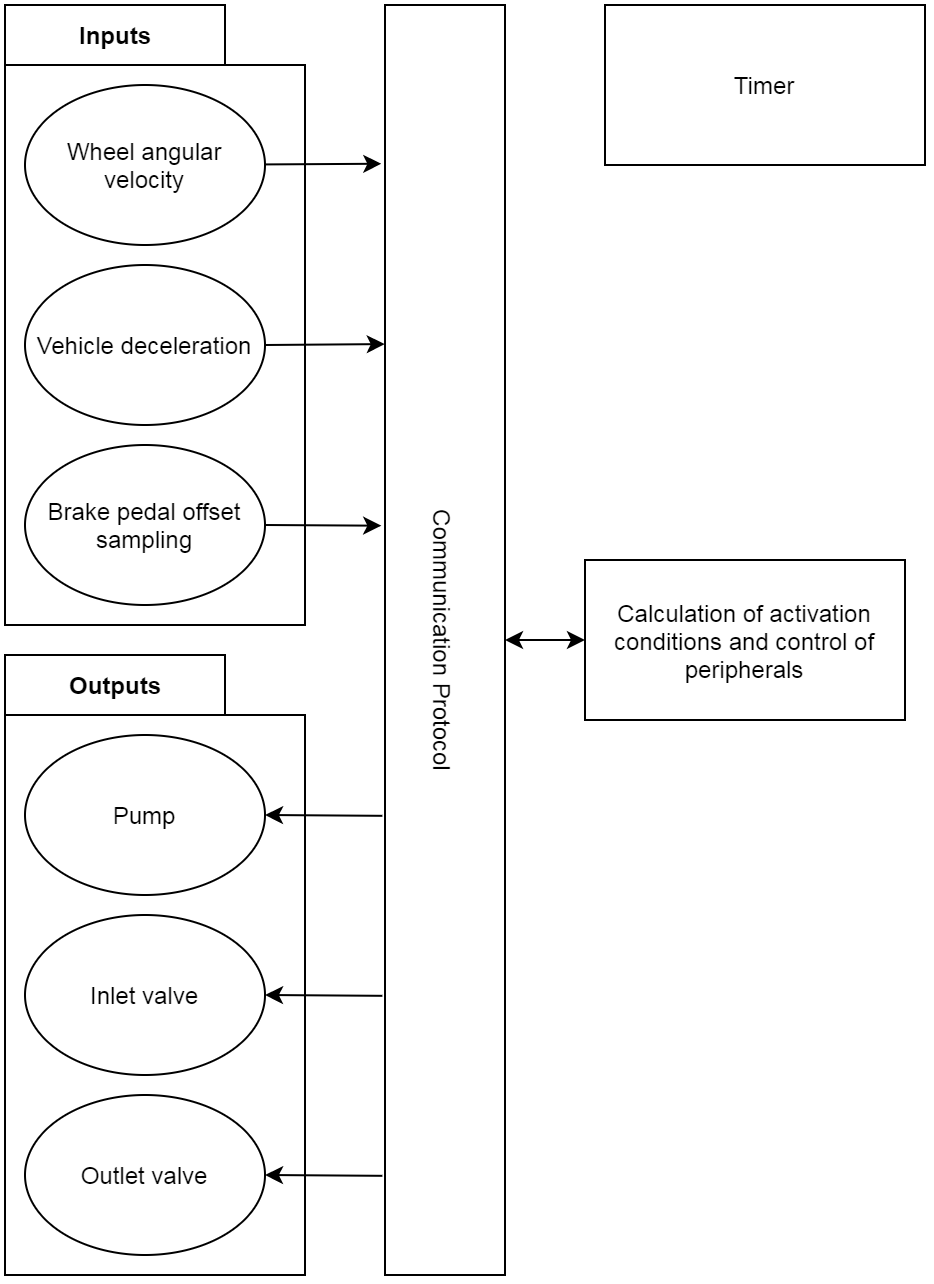
\includegraphics[scale=0.15]{images/software-architecture.png}}
  \end{figure}
\end{frame}

\begin{frame}
  \frametitle{Αρχιτεκτονική υλικού}
  \begin{figure}[h]
    \begin{center}
    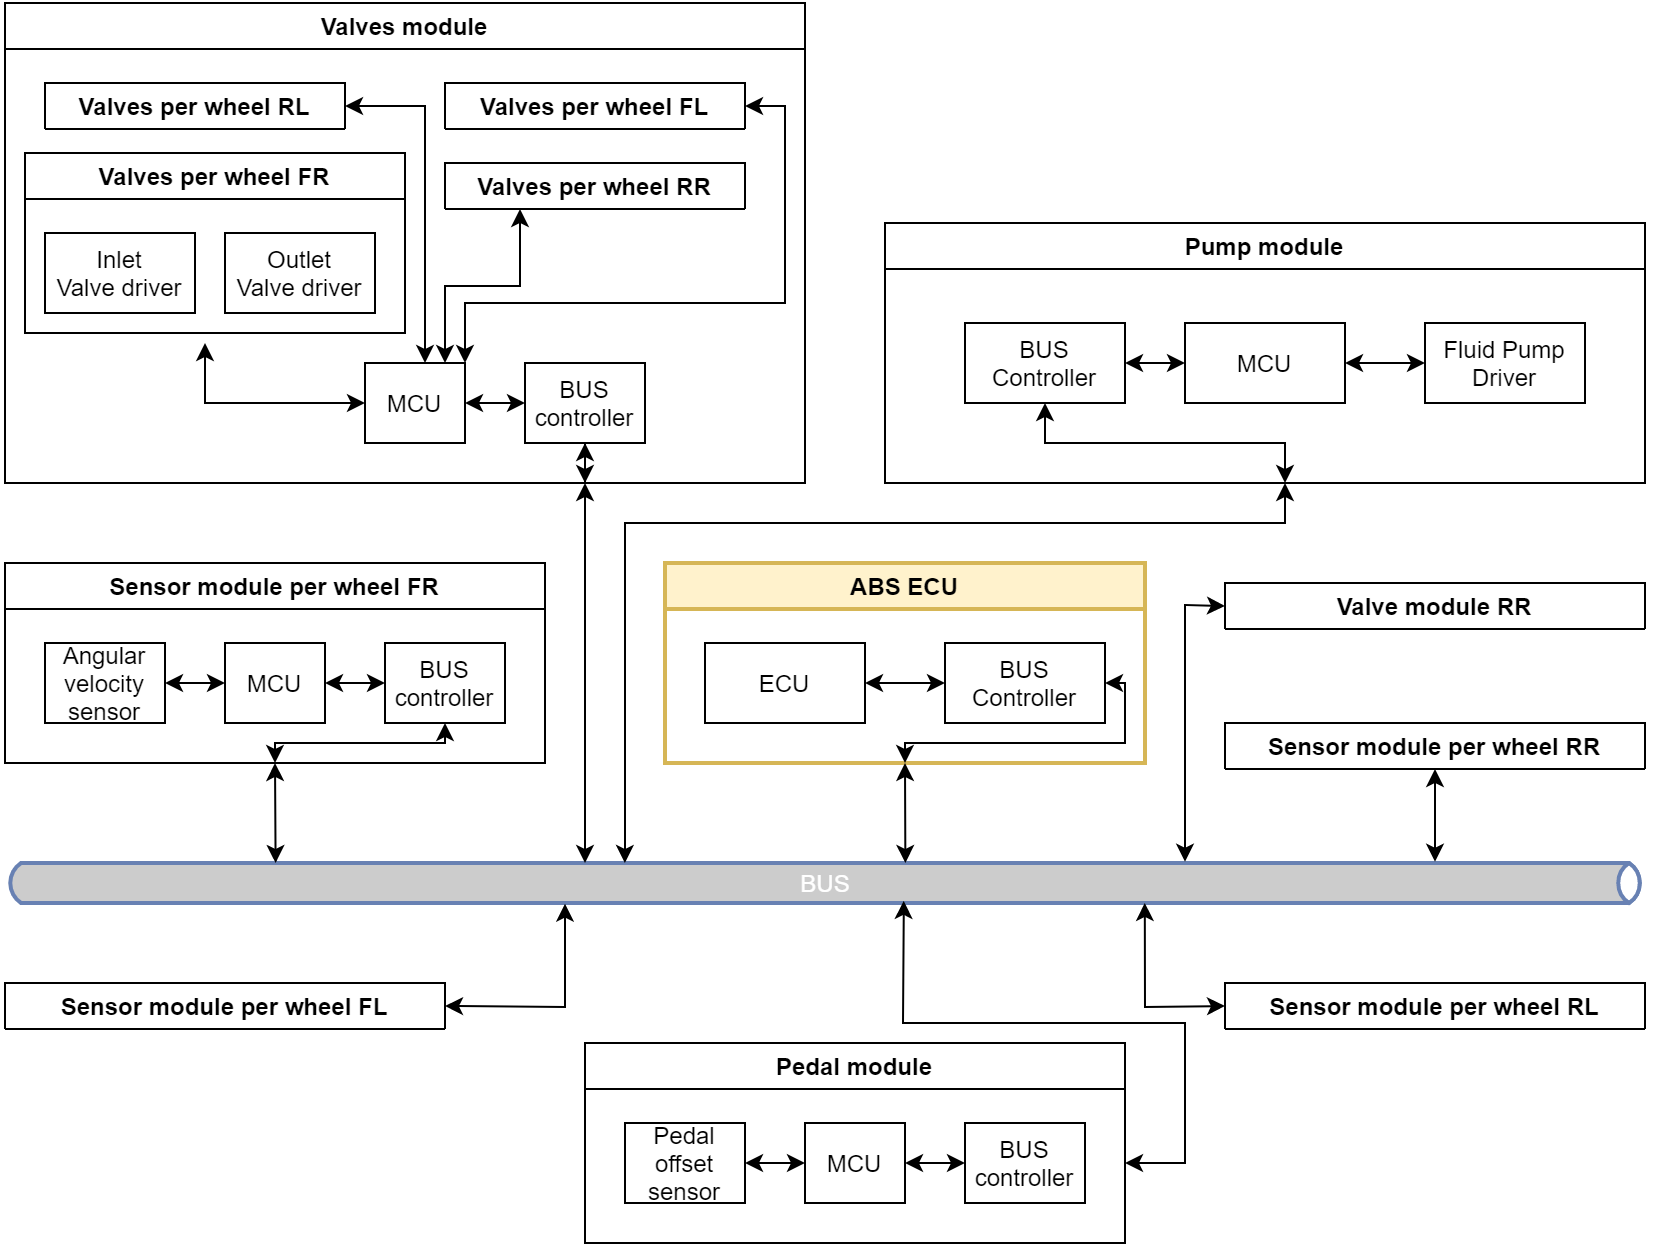
\includegraphics[scale=0.17]{images/hardware-architecture.png}
    \end{center}
\end{figure}
\end{frame}

\begin{frame}
  \frametitle{Σχεδιασμός υποσυστημάτων}
  Ο σχεδιασμός υποσυστημάτων περιλαμβάνει το:
  \begin{itemize}
    \item Υποσύστημα δίαυλου επικοινωνίας
    \item Υποσύστημα αισθητήρα τροχού
    \item Υποσύστημα πεντάλ φρένου
    \item Υποσύστημα βαλβίδων
    \item Υποσύστημα αντλίας
    \item Υποσύστημα ABS ECU
  \end{itemize}
\end{frame}

\begin{frame}
  \frametitle{Υποσύστημα διαύλου επικοινωνίας}
  \begin{itemize}
      \item Επιλέχθηκε το σύνολο πρωτοκόλλων CAN
  \end{itemize}
\begin{figure}[H]
    \begin{center}
    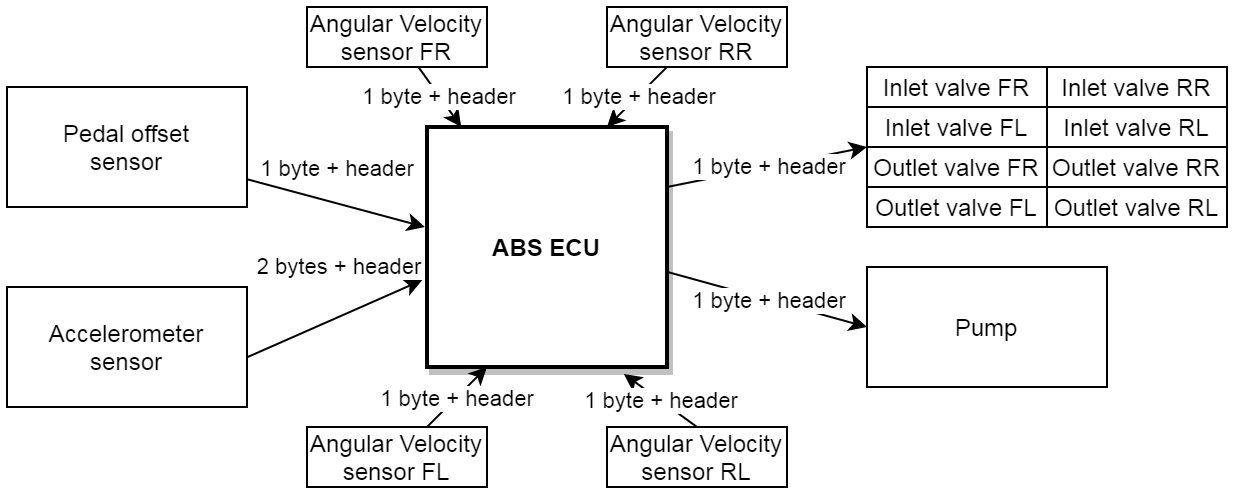
\includegraphics[scale=0.27]{images/inner-communications-v2.png}
    \end{center}
\end{figure}
\end{frame}

\begin{frame}
  \frametitle{Υποσύστημα αισθητήρα τροχού}
\begin{figure}[H]
    \begin{center}
    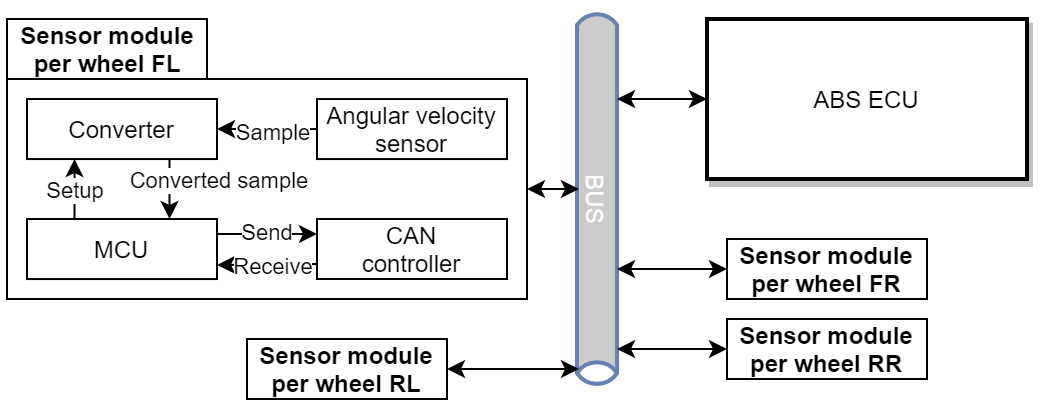
\includegraphics[scale=0.27]{images/angular-velocity-module-design.png}
    \end{center}
\end{figure}
\end{frame}

\begin{frame}
  \frametitle{Υποσύστημα πεντάλ φρένου}
  \begin{itemize}
      \item Το υποσύστημα αποτελείται από τα παρακάτω:
      \begin{itemize}
        \item Αισθητήρας φρένου
        \item Μετατροπέας ADC σήματος αισθητήρα
        \item Μικροελεγκτής
      \end{itemize}
  \end{itemize}
\end{frame}

\begin{frame}
  \frametitle{Υποσύστημα βαλβίδων-αντλιών}
  \begin{itemize}
    \item Το υποσύστημα βαλβίδων αποτελείται από:
      \begin{itemize}
        \item Βαλβίδες
        \item Μικροελεγκτής
      \end{itemize}
        \item Το υποσύστημα αντλιών αποτελείται από:
      \begin{itemize}
        \item Αντλία
        \item Ελεγκτής αντλίας
        \item Μικροελεγκτής
      \end{itemize}
  \end{itemize}
\end{frame}

\begin{frame}
  \frametitle{Υποσύστημα ABS ECU}
  \begin{itemize}
        \item Το υποσύστημα κεντρικής μονάδας επεξεργασίας:
\begin{figure}[H]
    \begin{center}
    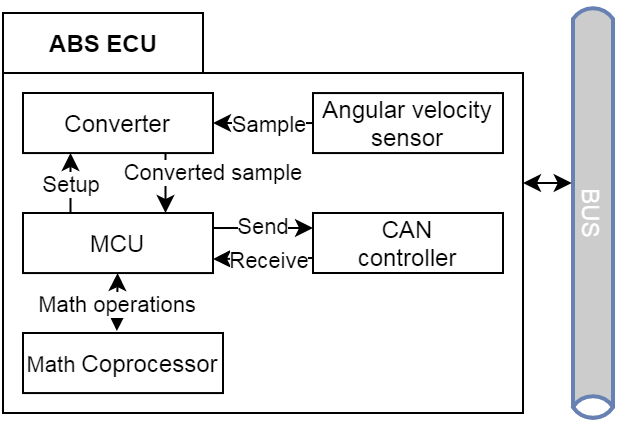
\includegraphics[scale=0.27]{images/central-abs-ecu-module-design.png}
    \end{center}
\end{figure}
  \end{itemize}

\end{frame}

\begin{frame}
  \frametitle{Πειραματική υλοποίηση}
  \begin{itemize}
      \item Επιλέχθηκε το επιταχυνσιόμετρο που περιέχεται στον ΜPU-9250
      \item Ελέγχθηκε η καταλληλότητα του σχετικά με τις σχεδιαστικές απαιτήσεις και διαπιστώθηκε ότι είναι ακατάλληλος
      \item Προγραμματίστηκε με χρήση ESP32 το οποίο επικοινωνούσε με τον αισθητήρα μέσω I\textsuperscript{2}C
      \item Παραμετροποιήθηκε ως εξής :
        \begin{itemize}
            \item Κλίμακα μέτρησης \tpm 4g (8 LSB/g)
            \item LPF με bandwidth 42Hz και sample rate 200Hz και 
            \item LPF με bandwidth 5Hz και sample rate 30Hz
        \end{itemize}
  \end{itemize}
\end{frame}

\begin{frame}{Πειραματική υλοποίηση}

\begin{figure}[H]
    \centering
    \subfigure{\textwidth}{
        \centering
        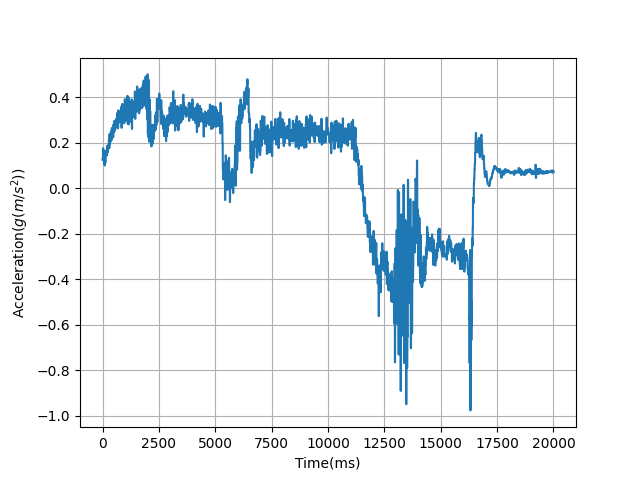
\includegraphics[width=0.49\textwidth]{images/samples_km45.txt.png}
        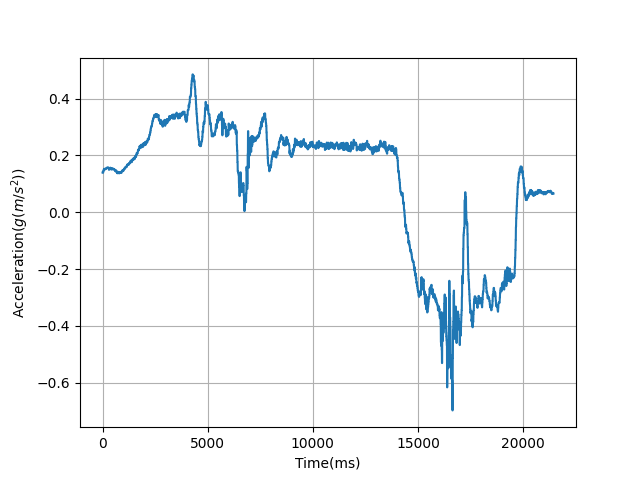
\includegraphics[width=0.49\textwidth]{images/samples_km45_hz5.txt.png}
        \caption*{Πειραματικές μετρήσεις επιβράδυνσης/χρόνου απότομης πέδησης από τελική ταχύτητα 40 km/h με 42KHz LPF (αριστερά) και με 5KHz LPF (δεξιά)}
    }
\end{figure}
\end{frame}

\begin{frame}
  \frametitle{Διαδικασίες ελέγχου ορθής λειτουργίας}
  \begin{itemize}
      \item Ελέγχθηκε η λειτουργία self-test που έχει ενσωματωμένη το επιταχυνσιόμετρο
      \item Χρήσιμη σε πιθανές βελτιώσεις του συστήματος
  \end{itemize}
  \begin{figure}[h]
    \begin{center}
    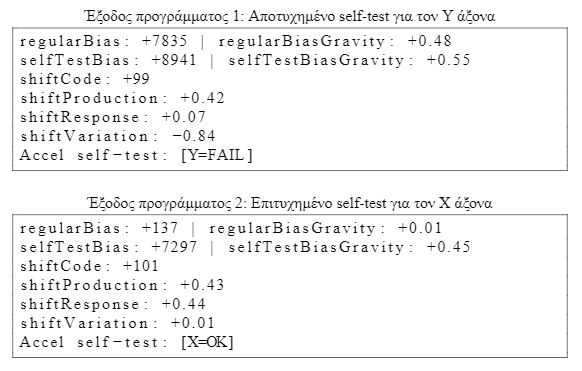
\includegraphics[scale=0.60]{images/self-test-log.png}
    \end{center}
\end{figure}
\end{frame}

\begin{frame}
  \frametitle{Βελτιστοποιήσεις και προτάσεις}
  \begin{itemize}
    \item Υποστήριξη ενδείξεων κακής λειτουργίας ή φθοράς μερών του συστήματος.
        \begin{itemize}
            \item Εκτέλεση ελέγχου κάθε φορά που τείθεται σε λειτουργία το αμάξι.
            \item Απλό πρωτόκολλο επικοινωνίας μεταξύ ABS ECU και υπόλοιπων υποσυστημάτων
            \item Υποστήριξη προτύπων διάγνωσης σφαλμάτων OBD από την ABS ECU
        \end{itemize}
    \item Χρήση ξεχωριστού διαύλου μόνο για την επικοινωνία μεταξύ της ABS ECU (π.χ. PSI-5)
        \begin{itemize}
            \item Βελτίωση στη περίπτωση οχημάτων με υπερφορτωμένο δίαυλο CAN
        \end{itemize}
  \end{itemize}
\end{frame}

\begin{frame}
\begin{center}
    Ευχαριστούμε
\end{center}
\end{frame}

\end{document}
